\section{Penyajian Data Uji Coba}

Pada penelitian ini dilakukan uji coba menggunakan data lokasi seluruh SMA di Kabupaten Probolinggo, dan dijalankan menggunakan python. Berikut adalah sajian data hasil uji coba.

\subsection{Pengambilan Data Lokasi}

Data yang digunakan adalah data koordinat lokasi yang diekspor memalui google earth. Pengujian Pengambilan data lokasi bertujuan untuk menunjukkan bahwa sistem 
mampu membaca input yang dimasukkan. Dapat dilihat pada Gambar \ref{fig:datalok} sebagian nama nama sekolah di kabupaten probolinggo beserta koordinat lokasinya.

\begin{figure}[h!]
  \centering
  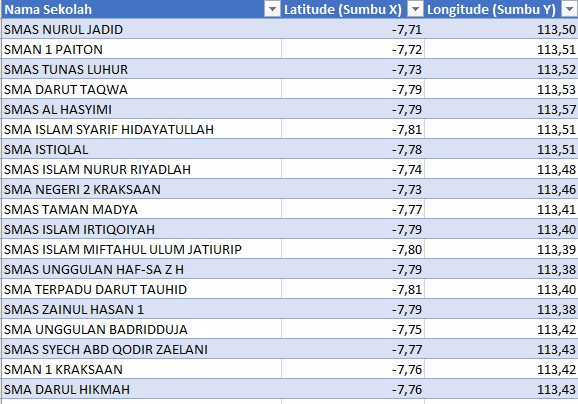
\includegraphics[width=0.8\textwidth]{data lokasi sekolah.png}
  \caption{Beberapa Data Lokasi Sekolah}
  \label{fig:datalok}
\end{figure}

Setelah mendapatkan lokasi yang akan diproses, selanjutnya adalah menentukan beberapa titik centroid secara random, dalam penelitian ini akan diambil 10 centroid secara random seperti pada gambar \ref{fig:dasen}.

\begin{figure}[h!]
	\centering
	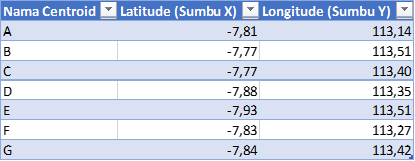
\includegraphics[width=0.8\textwidth]{centroid.png}
	\caption{Data Centroid}
	\label{fig:dasen}
\end{figure}

\subsection{Proses Pengklasteran Data}

Pada tahap ini metode yang digunakan adalah metode $K-$means untuk mengklaster data